% Options for packages loaded elsewhere
\PassOptionsToPackage{unicode}{hyperref}
\PassOptionsToPackage{hyphens}{url}
%
\documentclass[
  man]{apa6}
\usepackage{amsmath,amssymb}
\usepackage{lmodern}
\usepackage{iftex}
\ifPDFTeX
  \usepackage[T1]{fontenc}
  \usepackage[utf8]{inputenc}
  \usepackage{textcomp} % provide euro and other symbols
\else % if luatex or xetex
  \usepackage{unicode-math}
  \defaultfontfeatures{Scale=MatchLowercase}
  \defaultfontfeatures[\rmfamily]{Ligatures=TeX,Scale=1}
\fi
% Use upquote if available, for straight quotes in verbatim environments
\IfFileExists{upquote.sty}{\usepackage{upquote}}{}
\IfFileExists{microtype.sty}{% use microtype if available
  \usepackage[]{microtype}
  \UseMicrotypeSet[protrusion]{basicmath} % disable protrusion for tt fonts
}{}
\makeatletter
\@ifundefined{KOMAClassName}{% if non-KOMA class
  \IfFileExists{parskip.sty}{%
    \usepackage{parskip}
  }{% else
    \setlength{\parindent}{0pt}
    \setlength{\parskip}{6pt plus 2pt minus 1pt}}
}{% if KOMA class
  \KOMAoptions{parskip=half}}
\makeatother
\usepackage{xcolor}
\usepackage{longtable,booktabs,array}
\usepackage{calc} % for calculating minipage widths
% Correct order of tables after \paragraph or \subparagraph
\usepackage{etoolbox}
\makeatletter
\patchcmd\longtable{\par}{\if@noskipsec\mbox{}\fi\par}{}{}
\makeatother
% Allow footnotes in longtable head/foot
\IfFileExists{footnotehyper.sty}{\usepackage{footnotehyper}}{\usepackage{footnote}}
\makesavenoteenv{longtable}
\usepackage{graphicx}
\makeatletter
\def\maxwidth{\ifdim\Gin@nat@width>\linewidth\linewidth\else\Gin@nat@width\fi}
\def\maxheight{\ifdim\Gin@nat@height>\textheight\textheight\else\Gin@nat@height\fi}
\makeatother
% Scale images if necessary, so that they will not overflow the page
% margins by default, and it is still possible to overwrite the defaults
% using explicit options in \includegraphics[width, height, ...]{}
\setkeys{Gin}{width=\maxwidth,height=\maxheight,keepaspectratio}
% Set default figure placement to htbp
\makeatletter
\def\fps@figure{htbp}
\makeatother
\setlength{\emergencystretch}{3em} % prevent overfull lines
\providecommand{\tightlist}{%
  \setlength{\itemsep}{0pt}\setlength{\parskip}{0pt}}
\setcounter{secnumdepth}{-\maxdimen} % remove section numbering
% Make \paragraph and \subparagraph free-standing
\ifx\paragraph\undefined\else
  \let\oldparagraph\paragraph
  \renewcommand{\paragraph}[1]{\oldparagraph{#1}\mbox{}}
\fi
\ifx\subparagraph\undefined\else
  \let\oldsubparagraph\subparagraph
  \renewcommand{\subparagraph}[1]{\oldsubparagraph{#1}\mbox{}}
\fi
\newlength{\cslhangindent}
\setlength{\cslhangindent}{1.5em}
\newlength{\csllabelwidth}
\setlength{\csllabelwidth}{3em}
\newlength{\cslentryspacingunit} % times entry-spacing
\setlength{\cslentryspacingunit}{\parskip}
\newenvironment{CSLReferences}[2] % #1 hanging-ident, #2 entry spacing
 {% don't indent paragraphs
  \setlength{\parindent}{0pt}
  % turn on hanging indent if param 1 is 1
  \ifodd #1
  \let\oldpar\par
  \def\par{\hangindent=\cslhangindent\oldpar}
  \fi
  % set entry spacing
  \setlength{\parskip}{#2\cslentryspacingunit}
 }%
 {}
\usepackage{calc}
\newcommand{\CSLBlock}[1]{#1\hfill\break}
\newcommand{\CSLLeftMargin}[1]{\parbox[t]{\csllabelwidth}{#1}}
\newcommand{\CSLRightInline}[1]{\parbox[t]{\linewidth - \csllabelwidth}{#1}\break}
\newcommand{\CSLIndent}[1]{\hspace{\cslhangindent}#1}
\ifLuaTeX
\usepackage[bidi=basic]{babel}
\else
\usepackage[bidi=default]{babel}
\fi
\babelprovide[main,import]{english}
% get rid of language-specific shorthands (see #6817):
\let\LanguageShortHands\languageshorthands
\def\languageshorthands#1{}
% Manuscript styling
\usepackage{upgreek}
\captionsetup{font=singlespacing,justification=justified}

% Table formatting
\usepackage{longtable}
\usepackage{lscape}
% \usepackage[counterclockwise]{rotating}   % Landscape page setup for large tables
\usepackage{multirow}		% Table styling
\usepackage{tabularx}		% Control Column width
\usepackage[flushleft]{threeparttable}	% Allows for three part tables with a specified notes section
\usepackage{threeparttablex}            % Lets threeparttable work with longtable

% Create new environments so endfloat can handle them
% \newenvironment{ltable}
%   {\begin{landscape}\centering\begin{threeparttable}}
%   {\end{threeparttable}\end{landscape}}
\newenvironment{lltable}{\begin{landscape}\centering\begin{ThreePartTable}}{\end{ThreePartTable}\end{landscape}}

% Enables adjusting longtable caption width to table width
% Solution found at http://golatex.de/longtable-mit-caption-so-breit-wie-die-tabelle-t15767.html
\makeatletter
\newcommand\LastLTentrywidth{1em}
\newlength\longtablewidth
\setlength{\longtablewidth}{1in}
\newcommand{\getlongtablewidth}{\begingroup \ifcsname LT@\roman{LT@tables}\endcsname \global\longtablewidth=0pt \renewcommand{\LT@entry}[2]{\global\advance\longtablewidth by ##2\relax\gdef\LastLTentrywidth{##2}}\@nameuse{LT@\roman{LT@tables}} \fi \endgroup}

% \setlength{\parindent}{0.5in}
% \setlength{\parskip}{0pt plus 0pt minus 0pt}

% Overwrite redefinition of paragraph and subparagraph by the default LaTeX template
% See https://github.com/crsh/papaja/issues/292
\makeatletter
\renewcommand{\paragraph}{\@startsection{paragraph}{4}{\parindent}%
  {0\baselineskip \@plus 0.2ex \@minus 0.2ex}%
  {-1em}%
  {\normalfont\normalsize\bfseries\itshape\typesectitle}}

\renewcommand{\subparagraph}[1]{\@startsection{subparagraph}{5}{1em}%
  {0\baselineskip \@plus 0.2ex \@minus 0.2ex}%
  {-\z@\relax}%
  {\normalfont\normalsize\itshape\hspace{\parindent}{#1}\textit{\addperi}}{\relax}}
\makeatother

% \usepackage{etoolbox}
\makeatletter
\patchcmd{\HyOrg@maketitle}
  {\section{\normalfont\normalsize\abstractname}}
  {\section*{\normalfont\normalsize\abstractname}}
  {}{\typeout{Failed to patch abstract.}}
\patchcmd{\HyOrg@maketitle}
  {\section{\protect\normalfont{\@title}}}
  {\section*{\protect\normalfont{\@title}}}
  {}{\typeout{Failed to patch title.}}
\makeatother

\usepackage{xpatch}
\makeatletter
\xapptocmd\appendix
  {\xapptocmd\section
    {\addcontentsline{toc}{section}{\appendixname\ifoneappendix\else~\theappendix\fi\\: #1}}
    {}{\InnerPatchFailed}%
  }
{}{\PatchFailed}
\keywords{effect size, statistical power, executive function, implicit learning, attentional blink, multitasking, contextual cueing, serial response task\newline\indent Word count: 8873}
\DeclareDelayedFloatFlavor{ThreePartTable}{table}
\DeclareDelayedFloatFlavor{lltable}{table}
\DeclareDelayedFloatFlavor*{longtable}{table}
\makeatletter
\renewcommand{\efloat@iwrite}[1]{\immediate\expandafter\protected@write\csname efloat@post#1\endcsname{}}
\makeatother
\usepackage{lineno}

\linenumbers
\usepackage{csquotes}
\ifLuaTeX
  \usepackage{selnolig}  % disable illegal ligatures
\fi
\IfFileExists{bookmark.sty}{\usepackage{bookmark}}{\usepackage{hyperref}}
\IfFileExists{xurl.sty}{\usepackage{xurl}}{} % add URL line breaks if available
\urlstyle{same} % disable monospaced font for URLs
\hypersetup{
  pdftitle={Quantifying error in effect size estimates in attention, executive function and implicit learning},
  pdfauthor={*Kelly G. Garner1,3, Christopher R. Nolan2, Abbey Nydam3, Zoie Nott3, Howard Bowman1, \& Paul E. Dux3},
  pdflang={en-EN},
  pdfkeywords={effect size, statistical power, executive function, implicit learning, attentional blink, multitasking, contextual cueing, serial response task},
  hidelinks,
  pdfcreator={LaTeX via pandoc}}

\title{Quantifying error in effect size estimates in attention, executive function and implicit learning}
\author{*Kelly G. Garner\textsuperscript{1,3}, Christopher R. Nolan\textsuperscript{2}, Abbey Nydam\textsuperscript{3}, Zoie Nott\textsuperscript{3}, Howard Bowman\textsuperscript{1}, \& Paul E. Dux\textsuperscript{3}}
\date{}


\shorttitle{Quantifying error in effect size estimates}

\authornote{

*denotes corresponding author: \href{mailto:getkellygarner@gmail.com}{\nolinkurl{getkellygarner@gmail.com}}

This project has received funding from the European Union's Horizon 2020 research and innovation programme under the Marie Skłodowska-Curie grant agreement No 796329, awarded to Kelly Garner, and ARC Discovery Projects DP180101885 \& DP210101977 awarded to Paul Dux.

Correspondence concerning this article should be addressed to *Kelly G. Garner. E-mail: \href{mailto:getkellygarner@gmail.com}{\nolinkurl{getkellygarner@gmail.com}}

}

\affiliation{\vspace{0.5cm}\textsuperscript{1} School of Psychology, University of Birmingham, UK\\\textsuperscript{2} School of Psychology, University of New South Wales, Australia\\\textsuperscript{3} School of Psychology, The University of Queensland, Australia}

\begin{document}
\maketitle

Data: \url{https://doi.org/10.48610/b63ecc2} Garner \& Nolan (2022)

Code: \url{https://github.com/kel-github/Super-Effects} Garner, Knott \& Nolan (2022)

\clearpage

\hypertarget{abstract}{%
\section{Abstract}\label{abstract}}

Accurate quantification of effect sizes has the power to motivate theory, and reduce misinvestment of scientific resources by informing power calculations during study planning. However, a combination of publication bias and small sample sizes (\textasciitilde{}\(N\) = 25) hampers certainty in current effect size estimates. We sought to determine the extent to which sample sizes may produce error in effect size estimates for four commonly used paradigms assessing attention, executive function and implicit learning (Attentional Blink (AB), Multitasking (MT), Contextual Cueing (CC), Serial Response Task (SRT)). We combined a large data-set with a bootstrapping approach to simulate 1000 experiments across a range of \(N\) (13-313). Beyond quantifying the effect size and statistical power that can be anticipated for each study design, we demonstrate that experiments with lower \(N\) may double or triple information loss. We also show that basing power calculations on effect sizes from similar studies yields a problematically imprecise estimate between 40-67\% of the time, given commonly used sample sizes. Last, we show that skewness of inter-subject behavioural effects may serve as a predictor of an erroneous estimate. We conclude with practical recommendations for researchers and demonstrate how our simulation approach can yield theoretical insights that are not readily achieved by other methods; such as identifying the information gained from rejecting the null hypothesis, and quantifying the contribution of individual variation to error in effect size estimates.

\clearpage

\hypertarget{introduction}{%
\section{Introduction}\label{introduction}}

Despite the complexity involved in disentangling the processes that underpin cognition, decision making regarding experimental outcomes is often made on binary (i.e.~pass or fail) terms, across the psychological, neuroscientific and biomedical sciences (Szucs \& Ioannidis, 2017). Theoretical predictions are often specified in terms of the presence or absence of a given effect, and a yes/no decision is made about whether the null hypothesis (usually a hypothesis of null differences) can be rejected. It seems unlikely that such binary decision-making will be sufficient to disentangle the myriad functional systems that comprises the brain's processes. An alternate approach is to develop theory and models that predict the magnitude of the effect. \textcolor{blue}{Providing predictions in terms of effect size magnitude prompts theorists to consider the variability as well as the presence of predicted effects, and is demonstrably a useful metric when considering practical relevance} (Funder \& Ozer, 2019). Such magnitudes are often characterised as an effect size: a standardised measure that reflects the extent to which an effect, such as a mean difference between two conditions, is expected to generalise to the population (Cohen, 1988).

A prediction of effect magnitude is easier to disprove than a binary outcome, and therefore constitutes a more desirable prediction for theory testing (Popper, 1959). To move towards theories that predict changes in effect size magnitude, it is helpful to gain an understanding of how much insight is yielded from our current effect size estimates; i.e.~how well are we currently quantifying effect sizes, and should we increase sample sizes to quantify them better? Indeed, recent work suggests that insufficiently powered studies are at increased risk of producing effect size estimates that are either inflated in magnitude, or are in the incorrect direction (Chen et al., 2019; Gelman \& Carlin, 2014). Here we seek to address how well we currently characterise effect sizes in the study of cognition, using some established paradigms in the fields of attention, executive function and implicit learning; namely the Attentional Blink (AB, Raymond, Shapiro, \& Arnell, 1992), Multitasking (MT, Schumacher et al., 2001), Serial Response Task (SRT, Nissen \& Bullemer, 1987), and Contextual Cueing (CC, Chun \& Jiang, 1998) paradigms.

Accurate quantification of effect sizes is also desirable for study planning, as effect sizes form the foundation of \emph{a priori} power calculations (Cohen 1988). Here the researcher determines the sample size (\(N\)) required to achieve sufficient power to correctly reject the null hypothesis. The importance - and difficulty - of accurately determining the anticipated effect size has been considered extensively elsewhere (Cohen, 1988; Gelman \& Carlin, 2014; Albers \& Lakens, 2018; Cumming, 2014;, Egger, Smith, Schneider, \& Minder, 1997; Guo, Logan, Glueck, \& Muller, 2013; Lakens, 2013; Szucs \& Ioannidis, 2017; Westfall, Kenny, \& Judd, 2014). Standard approaches of determining an anticipated effect size involve consulting a meta-analysis, basing effect-size estimates on a few similar studies (incomplete sampling), or determining the smallest effect that is of theoretical relevance (e.g. Gelman \& Carlin, 2014). What remains somewhat less considered is the utility of knowing how effect size estimates may vary across replications of an experiment (e.g. Cumming, 2014; Lorca-Puls et al., 2018), i.e.~what are the distributional properties of the effect size, given a field that uses a comparable \(N\) across experiments?

The answer to this question can facilitate both study planning and theory development. A paradigm that elicits a small effect that manifests with low variability across replications may be considered a more desirable target for theory and model development than a paradigm that produces the same mean effect size but with wider variability. With regard to study planning, identifying the lower bound of an expected effect size facilitates computation of the \(N\) required to achieve sufficient statistical power under the worst case scenario (Gelman \& Carlin, 2014). Understanding how effect sizes vary across replications with a given \(N\) also allows computation of the likelihood that any single study has produced a reasonably accurate estimate, which can inform the researcher who may be computing anticipated effect sizes on the basis of one or a few similar studies. There is also utility in knowing to what extent variability in effect size observations reduces when larger \(N\) are used instead. There may be an upper bound on the accuracy with which a particular effect can be estimated, for example, when the construction of a paradigm introduces a certain level of noise or measurement error that is larger than variation at the level of the individual. Consequently, there may be a point of diminishing returns, where the cost of recruiting extra \(N\) will outweigh the gains in accuracy of effect size estimation.

Quantifying the range of effect sizes that may be observed across experimental replications is not trivial. Indeed, it has been noted that the largest challenge in experimental design is the prior identification of a plausible range of effect sizes (Gelman \& Carlin, 2014). Meta-analytic and incomplete sampling approaches for determining an expected effect size are hampered by the quality of the existing literature (Brand, Bradley, Best, \& Stoica, 2008; Friston, 2012; Gelman \& Carlin, 2014; Lane \& Dunlap, 1978; Lorca-Puls et al., 2018). A recent survey of 900 effect sizes across psychology disciplines showed that effects from non-pre-registered studies were much larger than pre-registered studies (\(r\) = 0.36 vs 0.16, Schäfer and Schwarz (2019)) suggesting that prior to pre-registration, under-powered studies were contributing inflated effect size estimates to the psychology literature. \textcolor{blue}{Although multiple correction methods have been developed within the meta-analytic framework to account for biases due to missing literature} (Schmidt \& Hunter, 2015)\textcolor{blue}{, they typically involve assumptions about the sources of missing data, which can never be fully tested} (McShane, Böckenholt, \& Hansen, 2016; Wiernik \& Dahlke, 2020)\textcolor{blue}{. Thus even if one were to define an expected effect size using corrected meta-analyses (if available), there is much to gain corroborating meta-analytic results with alternate methods that can guarantee a lack of bias in the available dataset.} It is also difficult to determine, on the basis of existing literature \textcolor{blue}{- such as when using meta-analysis-} how conclusions about effect sizes would differ if a given field of study was different, e.g.~how much published literature is likely to be missing if a larger \(N\) was used as standard?

Simulation studies offer the opportunity to ask how well a field is currently quantifying effect sizes, and how a field's estimate of an effect size would change with differing levels of statistical power. Typically, simulation studies generate data under some simplifying assumptions about the data generation process (e.g. Albers \& Lakens, 2018; Hedges, 1982; Lane \& Dunlap, 1978; Troncoso Skidmore \& Thompson, 2013; Westfall et al., 2014). Although this work is necessary for informing how effect size estimates behave under varying conditions where ground truth is known, it is challenging to anticipate all the complexities of data from the repeated-measures designs used across a range of phenomena and processes, such as in the study of attention, executive function and implicit learning. Such data are often not normally distributed and carry varying levels of covariance between conditions. Thus, there remains a question mark over the extent to which the results from simulation work generalizes to real-world data. An alternative method is to simulate experimental outcomes by bootstrapping smaller samples from larger, real data-sets (e.g. Lorca-Puls et al., 2018). This approach offers the opportunity to characterize the distributional qualities of effect sizes estimated from high-dimensional data-sets, using varying levels of \(N\), while maintaining ecological validity.

In the current study, we applied such a simulation approach to characterize effect size distributions yielded from the study of cognition. Participants (\(N\) = 313) completed a battery of cognitive tasks (AB, MT, SRT and CC) originally assembled to test the relationship between attention, executive function and implicit learning. For each paradigm, we simulated 1000 bootstrapped experiments across 20 \(N\)s ranging from 13 to 313. For each paradigm and from each set of simulations, we determined the impact of \(N\) on error in effect size estimates. We asked how much variability of effect size estimates changes as a function of \(N\), and sought to identify a point at which increasing \(N\) may offer lower gains for improving effect size estimates. We next determined how likely it is that a study will produce an effect size estimate with sufficiently low error, as a function of \(N\). \textcolor{blue}{We also} sought to determine the impact of \(N\) on the potential for missing literature for each paradigm, given the case of publication bias. \textcolor{blue}{Last, we identified data features that predict error in effect size estimates, beyond the mean and standard deviation measures of which they are a function. Such features may serve as a flag for whether data from a single experiment may be susceptible to error in effect size estimates. We focused on the skew and kurtosis of inter- and intra-subject effects, as such measures can bias mean and variance estimates when datasets violate normality assumptions, yet remain undiscussed in simulation studies that assume normality. The results motivate guidelines for study design and interpretation, not only for future AB, MT, SRT and CC studies, but also more broadly for the investigation of cognition}.

\hypertarget{methods}{%
\section{Methods}\label{methods}}

\label{sec:Method}

\hypertarget{participants}{%
\subsection{Participants}\label{participants}}

\label{sec:Participants}

The current study used a data set collected for a different \href{https://osf.io/nxysg}{pre-registered} project examining the relationship between executive function and implicit learning. This data set contains performance measures from \(N\) = 313 participants. Participants were undergraduate students, aged 18 to 35 years old (mean = 20.14 yrs, sd = 3.46). Of the total sample, 208 reported being female, and 269 reported being right handed. Participants received course credits as compensation. All procedures were approved by The University of Queensland Human Research Ethics Committee and adhered to the \href{https://www.nhmrc.gov.au/about-us/publications/national-statement-ethical-conduct-human-research-2007-updated-2018}{National Statement on Ethical Conduct in Human Research}.

\hypertarget{apparatus}{%
\subsection{Apparatus}\label{apparatus}}

\label{sec:Apparatus}

Experimental procedures were run on an Apple Mac Minicomputer (OS X Late 2014, 2.8 GHz Intel Core i5) with custom code using the Psychophysics toolbox (v3.0.14) (Brainard, 1997; Pelli, 1997) in Matlab v2015b. Participants completed 7 tasks; Attentional Blink (AB), Multitasking (MT), Contextual Cueing (CC), Serial Response Task (SRT), Visual Statistical Learning (VSL), Operation Span task and a Stop Signal Inhibition task. Only the data from the AB, MT, CC and SRT are reported here. We opted not to report the VSL, OSPAN or Stop Signal data as their design did not lend themselves to the computation of a standardised effect size.

\hypertarget{procedures}{%
\subsection{Procedures}\label{procedures}}

\label{sec:Procedures}

Across all tasks, participants sat approximately 57 cm from the monitor. An overview of the task procedures is presented in Figure \ref{fig:FigureParadigm}. Details regarding each of the task protocols are presented within each section below.

\begin{figure}

{\centering 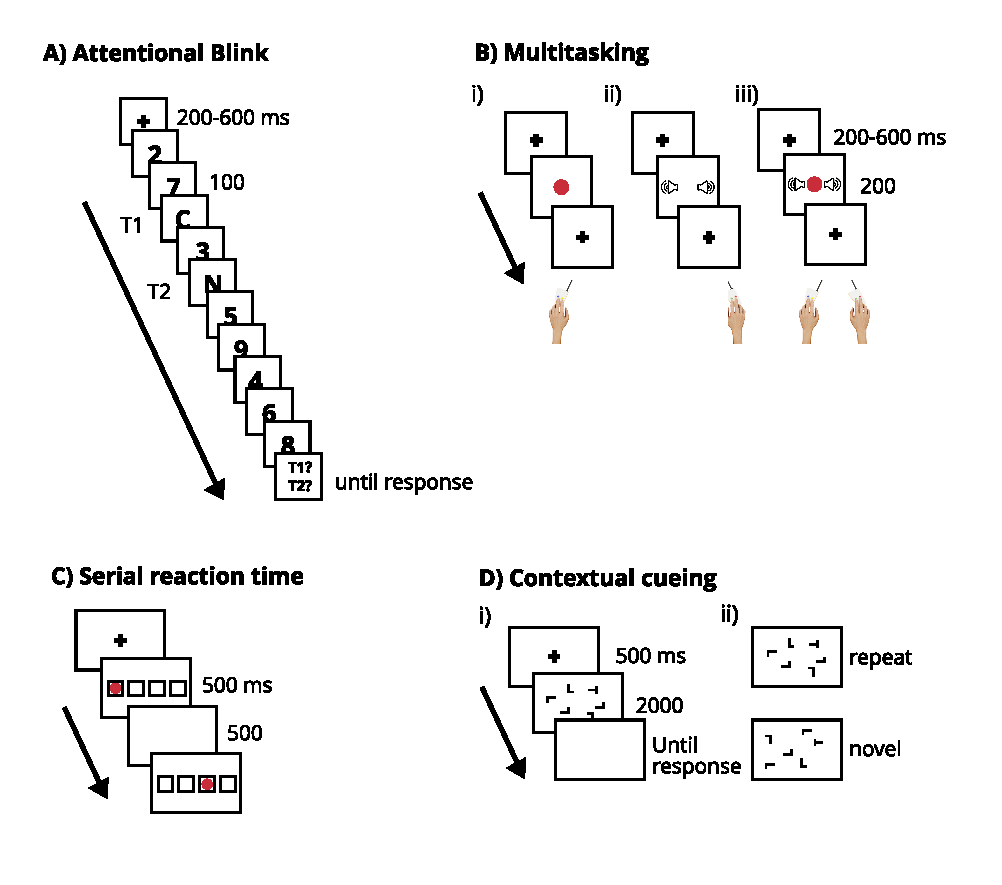
\includegraphics[width=0.7\linewidth]{../images/FigXXXX_alltasks} 

}

\caption{Task battery. A) Attentional Blink Paradigm (AB). Participants report the two letter targets from the rapid serial visual presentation of numbers and letters. B) Multitasking Paradigm (MT). Participants discriminate the colour of a disc, a complex tone, or both. C) Serial reaction time task (SRT). Participants respond to one of four stimuli, each mapped to a spatially-compatible button press. Unknown to participants, for half of the experimental blocks, the stimulus follows a repeating sequence. D) Contextual Cueing Paradigm (CC). i) Participants perform an inefficient visual search task where they search for a rotated T among L distractors. ii) Unknown to participants, half of the search arrays are repeated throughout the course of the experiment. }\label{fig:FigureParadigm}
\end{figure}

\hypertarget{attentional-blink-ab}{%
\subsubsection{Attentional Blink (AB)}\label{attentional-blink-ab}}

\label{sec:ABMeth}

The AB task taps limitations in the deployment of visual information processing over time. Participants are instructed to detect two targets from a rapidly presented series of visual items. Accuracy for the second target is poorer if it appears closer in time to the first target (at early lags, from lag 2 onwards), relative to further apart in time (Raymond et al., 1992).

\hypertarget{protocol}{%
\paragraph{Protocol}\label{protocol}}

The AB protocol was the same as that reported in Bender et al (2016). Each trial began with a black fixation cross in the center of a gray screen {[}RGB: 128, 128, 128{]} for a variable interval of 200-600 ms. On each trial, letter targets and digit distractors were presented centrally for 100 ms in rapid serial presentation. The eight distractors were drawn without replacement from the digits 2-9. The target letters were randomly selected from the English alphabet, excluding I, L, O, Q, U, V and X. The first target (T1) was presented third in the series (serial position 3), and T2 was presented at either lag 2 (200 ms), 3 (300 ms), 5 (500 ms) or 7 (700 ms) relative to T1. All stimuli subtended 1.72 x 2.31 \(^\circ\) (w x h) visual angle. Participants were instructed to make an unspeeded report of the identity of both targets at the end of each trial. Participants completed 24 practice trials and four test blocks of 24 trials. For the current analysis we calculated T2 accuracy, given that T1 was correctly reported (T2\textbar T1), for each lag.

\hypertarget{multitasking-mt}{%
\subsubsection{Multitasking (MT)}\label{multitasking-mt}}

\label{sec:MTMeth}

MT paradigms tap the performance costs incurred when individuals attempt to perform more than one task concurrently. Participants are instructed to complete two simple sensorimotor tasks as accurately and quickly as possible under single or multitask conditions. RTs to the constituent tasks are typically slowed for multitask relative to single task conditions (see Pashler (1994), for a review).

\hypertarget{protocol-1}{%
\paragraph{Protocol}\label{protocol-1}}

The MT protocol was previously reported in Bender et al (2016). Each trial began with a black fixation cross presented in the center of a gray screen {[}RGB: 128, 128, 128{]} for a variable interval of 200-600 ms. Next either one of two coloured circles {[}red, RGB: 237, 32, 36 or blue, RGB: 44, 71, 151{]} or one of two sounds (complex tones taken from Dux, Ivanoff, Asplund, \& Marois, (2006)), or both (circle and sound) were presented for 200 ms. The coloured circle subtended 1.3\(^\circ\) visual angle. Participants were instructed to respond to all tasks as quickly and accurately as possible, by using the appropriate key presses {[}`A' or `S' for left hand responses, `J' or `K' for right hand responses, with the task-hand mapping counterbalanced across participants{]}. The MT protocol consisted of 4 blocks of 36 trials, with each trial type (single-task {[}ST{]} visual, ST auditory or MT) randomly mixed within blocks. Participants completed the MT protocols after completing two ST blocks as practice, one for the visual task and one for the auditory task. We analysed mean response times (RTs) to each task x modality condition.

\hypertarget{serial-response-task-srt}{%
\subsubsection{Serial Response Task (SRT)}\label{serial-response-task-srt}}

\label{sec:SRTMeth}

The SRT paradigm taps sensorimotor sequence learning; specifically the extent to which individuals speed up responses when cue stimuli follow a predictable sequence, relative to when cue stimuli are presented randomly (Nissen \& Bullemer, 1987). As participants receive no explicit instructions or cues regarding the sequence, it has been assumed that the SRT taps implicit sequence learning (Nissen \& Bullemer, 1987), although the extent to which performance gains reflect implicit or explicit learning mechanisms continues to be debated (Clegg, DiGirolamo, \& Keele, 1998; Goschke, 1998). Participants are instructed to make a button press response to one of four spatially compatible target stimuli as quickly and accurately as possible. Unknown to the participants, the presentation of the target stimuli will on occasions follow a repeating rather than a random sequence.

\hypertarget{protocol-2}{%
\paragraph{Protocol}\label{protocol-2}}

The SRT was adapted from Nissen \& Bullemer (1987). Four square placeholders were presented across the horizontal meridian. A red circle {[}RGB: 255, 0, 0{]} appeared in one of the 4 squares for 500 ms. This served as the target stimulus. Participants responded by pressing the finger of their dominant hand that spatially aligned to the target circle, using the relevant `j', `k', `l' or `;' keys. The subsequent target stimulus appeared 500 ms after a correct response had been made. Participants completed 4 blocks of 100 trials. For blocks 1 and 4, the location of the target stimulus for each trial was randomly selected from a uniform distribution. These blocks are referred to as `Random'. For blocks 2 and 3, a repeating sequence of 10 elements was used to determine the target location. The sequence was repeated 10 times. The repeating sequence was 4-2-3-1-3-2-4-2-3-1, with 1 being the leftmost placeholder, and 4 being the rightmost placeholder. These blocks are referred to as `Sequence' blocks. Learning in the SRT is tested by comparing mean RTs between Sequence and Repeat blocks in the latter half of the experiment (block 4 vs 3).

\hypertarget{contextual-cueing-cc}{%
\subsubsection{Contextual Cueing (CC)}\label{contextual-cueing-cc}}

\label{sec:CCMeth}

CC tasks tap how the visual system exploits statistical regularities to guide visual search (Sisk, Remington and Jiang, (2019); Jiang and Sisk (2020)). Participants are typically asked to report the orientation of a rotated `T' target presented among an array of distractor 'L's. Participants are not informed that a set of the displays are repeated throughout the course of the experiment, while the remaining displays are novel to each trial. Typically RTs to the repeat displays become faster than novel displays throughout the course of the experiment (e.g. Chun \& Jiang, 1998; Nydam, Sewell, \& Dux, 2018). Participants are typically poor at recognising repeat displays in a subsequent recognition test (Sisk, Remington and Jiang, (2019); Jiang and Sisk (2020)), which has prompted the conclusion that CC reflects a process of implicit learning (but see Vadillo, Konstantinidis, \& Shanks, 2016; Vadillo, Linssen, Orgaz, Parsons, \& Shanks, 2020; Vadillo, Malejka, Lee, Dienes, \& Shanks, 2021).

\hypertarget{protocol-3}{%
\paragraph{Protocol}\label{protocol-3}}

The CC protocol was the same as that reported by Nydam et al (2018) which is modeled on Chun and Jiang (1998). Each trial began with a white fixation cross presented on a grey screen {[}RGB: 80, 80, 80{]}. An array of 12 L's and a single T were then presented presented within an invisible 15 x 15 grid that subtended 10\(^\circ\) x 10\(^\circ\) of visual angle. Orientation of each L was determined randomly to be rotated 0\(^\circ\), 90\(^\circ\), 180\(^\circ\) or 270\(^\circ\) clockwise. The T was oriented to either 90\(^\circ\) or 270\(^\circ\). Participants reported whether the T was oriented to the left (using the `z' key) or the right (using the `m' key), as quickly and accurately as possible. The task consisted of 12 blocks of 24 trials. For half the trials in each block, the display was taken (without replacement) from 1 of 12 configurations that was uniquely generated for each participant, where the location of the distractors and target (but not the orientation of the target) was fixed. These trials were called `repeats'. For the remaining trials, the display was randomly generated for each trial, making them `novel'. Displays were generated with the constraint that equal items be placed in each quadrant and each eccentricity. Target positions were matched between the repeat and novel displays for both quadrant and eccentricity. The exact location of the item was jittered within each cell for each presentation, to prevent perceptual learning or adaptation to the specific position of the item. The order of display type (repeat vs novel), configuration (1:12) and target orientation (left or right) was randomised for each block. Mean RTs to each block (1:12) and display type (repeat vs novel) were taken as the dependent variable.

\hypertarget{statistical-approach}{%
\subsection{Statistical Approach}\label{statistical-approach}}

All the \href{https://doi.org/10.48610/b63ecc2}{data} and \href{https://github.com/kel-github/Super-Effects}{code} used for the current analyses are available online. All data were analysed using R -Team (2015) and RStudio (RStudio Team, 2020). The analysis of the data from each task followed two steps; first, to ascertain that we observed the typical findings for each of the paradigms, we applied the relevant conventional statistical model to the full dataset (\(N\)=313). Next, we implemented a simulation procedure to determine the effect sizes and p-values that would be attained over many experiments conducted at multiple levels of sample size.

\hypertarget{simulation-procedure}{%
\subsubsection{Simulation procedure}\label{simulation-procedure}}

\label{sec:SamplingProc}

For each paradigm, we simulated experiments across 20 different sample sizes (\(N\)), defined on a logarithmic interval between \(N_{13}\) and \(N_{313}\) (\(N\) = {[}13, 15, 18, 21, 25, 30, 36, 42, 50, 59, 69, 82, 97, 115, 136, 160, 189, 224, 265, 313{]}). We opted for a logarithmic interval given that changes in effect size variability should be greater across changes of \(N\) when \(N\) is lower, relative to when \(N\)s are higher. To simulate \(k\)=1000 experiments at each of our chosen \(N\), we sampled \(N\) participants from \(N_{max}\) (\(N_{313}\)) over \(k\) iterations. The relevant analysis was applied to each of the samples. Details regarding which analyses were applied to each \(k\) sample are listed below for each paradigm. Sampling with replacement ensured that the samples carried the Markov property. One potential concern is that any reductions in observed effect size variability may be attributable to saturation as the simulated \(N\) approaches the maximum (\(N_{313}\)), rather than a genuine reduction in variance of the estimate of the effect. Specifically, it could be that as \(N\) approaches 313, the overlap of participants between samples is greater than when \(N\) equals a lower number such as 13. It follows then that any decreasing variability in effect size estimates at higher \(N\)s could be due to the decrease in variability of the samples, rather than the improved estimate of the population variance that should come with a larger \(N\). We have run simulations that argue against this explanation (see appendix i).

\hypertarget{effect-sizes}{%
\subsubsection{Effect Sizes}\label{effect-sizes}}

For each paradigm, we report the following information from the simulated effect size distributions; first we used simulations using \(N_{313}\) to provide a best estimate of the effect size distribution. We therefore report, for each paradigm, the mean (\emph{M}), median (\emph{Mdn}: when different to the \emph{M}), standard deviation (\emph{SD}), the .025 (lower bound, \emph{LB}) and .975 (upper bound, \emph{UB}) quantiles. These values can be used to define, \emph{a priori}, the range of anticipated effect sizes for future experiments, and consequently, can be used to inform study design.

We next determined to what extent using an \(N\) that is typical for the field impacts the effect size distribution. We report the same summary statistics as above, from the simulation using the \(N\) that is closest to the typical \(N\) for that task (\(N_{med}\)). To identify the typical \(N\), we conducted a survey of the recent literature and computed the median \(N\) for each paradigm (see below). We next computed the \emph{precision loss} incurred from using \(N_{med}\) by taking the ratio of the difference between the LB and UB quantiles for \(N_{med}\) and \(N_{313}\):

\[
qq{\text -}ratio = \frac{ UB_{N_{med}} - LB_{N_{med}}}{UB_{N_{313}} - LB_{N_{313}}}
\]

We refer to this measure from now as the qq-ratio. The qq-ratio indicates how under- or over-inflated effect size estimates may be - a qq-ratio of 2 would suggest that effect sizes may be twice as low or high as the LB or UB of the best estimate. For each task, we also report the largest observed qq-ratio and the \(N\) for which the qq-ratio reaches less than double. Note that although we expect qq-ratios to decrease as some function of \(\frac{1}{N}\) (given that variance depends on this term), the exact relationship between \(N\) and precision loss will be dependent on population variance and measurement error for any given paradigm. We also present qq-ratios across all \(N\)'s, to provide an idea of potential precision gains from increasing sample size.

Next we computed estimates regarding the extent to which precision loss in effect size estimates may lead a researcher awry during study planning. To determine how often sampling one or two similar studies with \(N_{med}\) may induce biases in power calculations, we computed for each task and \(N\), the proportion of simulated observations that fell within the LB and UB quantiles of the best estimate (\(N_{313}\)). This provides the probability that sampling one study will provide an accurate estimate of the true effect size. We refer to this as the probability of attaining a hit, given the sample size (p(hit\textbar{}\(N_{x}\))). (As above, although we expect this to change as a function of \(\frac{1}{N}\), the exact relationship is dependent on measurement noise). We next estimate effect size biases that result from aggregating across experiments with statistically significant results (p\textless.05), under the assumption that the published literature is more likely to only contain significant findings. We computed the difference between the mean effect size from significant results and the mean effect size from all results, and refer to this value as the \emph{inflation bias}. Effectively, this analysis is assessing the severity of the file-drawer effect for different sizes of \(N\). To inform understanding of potential file-drawer effects, we also report the proportion of studies that rejected the null hypothesis (\(p\) \textless{} .05) for \(N_{med}\), and the \(N\) where this value reached 90\% (note: this is related to the observed effect size, but we report it here for clarity).

\textcolor{blue}{Last, we sought metrics that may inform whether an experiment has yielded an imprecise effect size estimate. Effect sizes are a function of the variability of the effect across individuals, as well as intra-individual variability over trials} (Rouder \& Haaf, 2018). \textcolor{blue}{If either of these stem from a non-normal distribution, mean and standard deviation estimates -and consequently effect size computations- may be impacted. We thus determined whether the skewness and kurtosis of this data could predict error in effect size estimates.}

\textcolor{blue}{Error in effect sizes were defined for each task as the difference between the expected value for $N_{313}$ and each observed effect size from $N_{med}$. To attain predictors for each $N_{med}$ simulation, we calculated the key behavioural effect for each participant (in raw units) and computed the Pearson's skewness and kurtosis coefficients of the resulting distribution of effects. We also computed the variability, skew and kurtosis from each participant's performance across trials, and took the means of these measures across participants. The resulting variables (effect skewness, effect kurtosis, mean intra-individual variance, skewness, and kurtosis) served as predictors in a multiple regression analysis, using effect size error as the criterion variable. If any of the regressors themselves showed high levels of skew then a log transformation was applied. All model residuals were checked for homoscedasticity. Note that although we present the full models below, performing stepwise regression yielded the same pattern of results.}

\textcolor{blue}{To protect against interpreting over-fitted models, we performed k-fold cross-validation for each multiple regression model, where k=10, and we report the mean} \(r_{cv}^2\) \textcolor{blue}{ (and standard deviation) across folds. Next, we determined which regressors consistently predicted effect size error across the four tasks. We then sought to identify which values of such predictors suggest a problematic effect size error (defined as effect size errors that were less or more than the .025 and .975 quantiles for} \(N_{313}\) \textcolor{blue}{). We achieved this using simple regression, as we sought to simulate how much variability may be accounted for when a researcher uses a single piece of information to estimate effect size imprecision.}

\hypertarget{computing-effect-sizes}{%
\paragraph{Computing Effect Sizes}\label{computing-effect-sizes}}

To compute effect sizes for the paradigms analysed using a repeated-measures ANOVA (AB, MT and CC), we computed partial epsilon squared (\(\epsilon_{p}^2\)), as this measure is unbiased, unlike \(\eta_{p}^2\) (Okada, 2013). (Indeed, an earlier version of our manuscript showed that \(\eta_{p}^2\) estimates are biased on average, even for sample
sizes of \(N\)=313, \footnote{See for Supplemental Figures documenting this analysis: \url{https://github.com/kel-github/Super-Effects/tree/master/doc/supp-figs}. Note: we thank a helpful reviewer for drawing our attention to this}). We use the formula for \(\epsilon_{p}^2\) as defined in (Carroll \& Nordholm, 1975, eq 11):

\begin{equation}
\epsilon_{p}^{2} = \frac{F-1}{F + \frac{df_w}{df_b}}
\end{equation}

where \(F\) is the F statistic for the effect, \(df_{w}\) is the degrees of freedom within groups, and \(df_{b}\) is the degrees of freedom between groups. The SRT paradigm instead uses a paired-samples design. For this paradigm we computed Cohen's \(d_{z}\) (see Lakens (2013), eq 6):

\begin{equation}
d_{z} = \frac{M_{diff}}{\sqrt{\frac{\sum(X_{diff} - M_{diff})^2}{N-1}}}
\end{equation}

where \(M_{diff}\) is the mean difference between groups, and \(X_{diff}\) is the difference score for one subject.

To facilitate our interpretation of effect sizes as small, medium or large, we refer to Cohen (1992) for \(\epsilon_{p}^2\) and to Gignac \& Szodorai, (2016) for \(d_z\).

\hypertarget{representative-n}{%
\paragraph{Representative N}\label{representative-n}}

To attain an \(N\) that reflects what is commonly used for each paradigm, we surveyed the three most relevant \emph{Journal of Experimental Psychology} journals (\emph{General}, \emph{Human Perception \& Performance} and \emph{Learning, Memory \& Cognition}) for all articles mentioning use of any of the current paradigms. We searched back for a total of 60 experiments or back from today to 2005, whichever occurred first. We then computed the median sample size used across all experiments found from the survey. The results from the survey are presented in Table 1.

\begin{longtable}[]{@{}lcc@{}}
\caption{\label{tab:survey}Typical N found from literature survey. n exp = number or experiments, med N = median N}\tabularnewline
\toprule()
task & n exp & med N \\
\midrule()
\endfirsthead
\toprule()
task & n exp & med N \\
\midrule()
\endhead
AB & 60 & 24 \\
MT & 60 & 40 \\
CC & 49 & 24 \\
SRT & 60 & 34 \\
\bottomrule()
\end{longtable}

\hypertarget{analysis-of-experimental-tasks}{%
\subsubsection{Analysis of Experimental Tasks}\label{analysis-of-experimental-tasks}}

\hypertarget{attentional-blink}{%
\paragraph{Attentional Blink}\label{attentional-blink}}

As is typical for the field, and to ascertain the effectiveness of the lag manipulation, T2\textbar T1 accuracy was subject to a repeated measures ANOVA, with lag (2, 3, 5, \& 7) as the independent variable. This analysis was also applied to each \(k\) sample. For each \(k\) sample, \(\epsilon_{p}^2\) and the resulting \(p\) value were taken for the main effect of lag. For this task, and all remaining ANOVA tests, models were fit using the anova\_test() function from the \href{https://rpkgs.datanovia.com/rstatix/index.html}{rstatix} package. Where possible, the models were fit using type 3 sum of squares, owing to the computational expediency and match to commercial statistical software packages. In some cases, models were unable to be fit using type 3 sum of squares, owing to rank deficiencies in the underlying design matrix (e.g.~when one participant was drawn more than twice within a sample). In these cases, models were fit using type 1 sum of squares. However, as the experiment designs were fully balanced, each sum of squares type should yield the same results.

\hypertarget{multitasking}{%
\paragraph{Multitasking}\label{multitasking}}

To ascertain the effectiveness of the multitasking manipulation, the data were modelled using a 2 (task-modality: visual-manual vs auditory-manual) x 2 (task: ST vs MT) repeated-measures ANOVA. This analysis was also applied to each \(k\) sample; \(\epsilon_{p}^2\) and \(p\) are reported for both the main effect of task and the task-modality x task interaction.

\hypertarget{serial-response-task}{%
\paragraph{Serial Response Task}\label{serial-response-task}}

To ascertain whether participants learned the repeating sequences, RTs in the final block of sequence trials (block 3) were compared to those in the final block of random trials (block 4) using a paired-samples t-test. This analysis was also applied to each \(k\) sample, and we present the resulting Cohen's \(d_{z}\), and \(p\) value from each test.

\hypertarget{contextual-cueing}{%
\paragraph{Contextual Cueing}\label{contextual-cueing}}

To ascertain whether participants became faster for repeat relative to novel trials over the course of the experiment (i.e.~whether participants learned the statistical regularities of the repeated displays), the data were subject to a block (1:12) x condition (repeat vs novel display) repeated measures ANOVA. Specifically, learning should be evidenced by a significant block x condition interaction. This analysis was applied to each \(k\) sample, and we report \(\epsilon_{p}^2\) and \(p\) for the block x condition interaction.

As some studies from the contextual cueing literature suggest that the effect is better characterised by a main effect of condition thereby implying rapid learning of the statistical regularities (e.g. Peterson \& Kramer, 2001; Travis, Mattingley, \& Dux, 2013), we also report the \(\epsilon_{p}^2\) and \(p\) for the main effect of condition.

\hypertarget{results}{%
\section{Results}\label{results}}

\label{sec:Results}

We first present the results from the standard analyses used for each task, to show that we replicate the classic findings from each task. The key behavioural data are presented in Figure \ref{fig:behavResults}.

\begin{figure}

{\centering \includegraphics[width=0.7\linewidth]{../images/EPS_all_tasks_behav} 

}

\caption{Behavioural Results. A) Attentional Blink Paradigm (AB). Accuracy (acc) for T2|T1 was lower at early lags, relative to later lags. Note that T1 accuracy is also plotted. B) Multitasking Paradigm (MT). RTs were slowed for multitask (M) conditions, relative to single-tasks (S). This difference was larger for sound tasks (So) than for visual (V) tasks. C) Serial Response Task (SRT). In the second half of the experiment, RTs were faster in the sequence (S) relative to the random (R) condition. D) Contextual Cueing (CC). RTs were faster for the repeat (R) than for the novel (N) displays, and this difference became larger throughout the course of the experiment.}\label{fig:behavResults}
\end{figure}

\hypertarget{behavioural-results}{%
\subsection{Behavioural Results}\label{behavioural-results}}

\hypertarget{attentional-blink-1}{%
\subsubsection{Attentional Blink}\label{attentional-blink-1}}

\label{sec:ABRes}

The AB data are presented in Figure \ref{fig:behavResults}A. Accuracy for T2\textbar T1 was lower for early relative to late lags; accuracy for T2\textbar T1 decreased (by around p = 0.32) when T2 was presented at lag 2, relative to lag 7. A one-way ANOVA revealed that the effect of lag was statistically significant (F (2.4, 749) = 508, \(\epsilon_{p}^2\) = 0.62, p = 1.88e-157). Post-hoc t-tests showed that accuracy at each lag differed statistically from accuracy at each of the other lags (all p's \(\leq\) 3.68e-18). Therefore, the AB paradigm yielded the typically observed effects.

\hypertarget{multitasking-1}{%
\subsubsection{Multitasking}\label{multitasking-1}}

As anticipated, RTs were slowed for multitask relative to single task conditions (see Figure \ref{fig:behavResults}B). Mean RTs were on average 0.31 (95\% CI{[}0.30, 0.33{]}) seconds (s) slower on MT trials (F(1, 312) = 2653, \(\epsilon_{p}^2\) = 0.89, p\textless.0001). There was also a significant task modality (sound or visual) x task (ST vs MT) interaction (F(1, 312) = 59.4, \(\epsilon_{p}^2\) = 0.16, p\textless.0001). The MT cost (MT RT - ST RT) was larger for the sound task relative to the visual task by on average 0.08 s (95\% CI{[}0.06, 0.10{]}). This latter finding has been reported previously (Hazeltine \& Ruthruff, 2006). We continue to interrogate this effect, as it serves as an example of an interaction with a small effect size. This facilitates comparisons to the contextual cueing task, as reported below.

\hypertarget{srt}{%
\subsubsection{SRT}\label{srt}}

The results from the SRT paradigm are presented in Figure \ref{fig:behavResults}C. Participants learned the repeating sequence; RTs were on average 0.049 s faster (95\% CI {[}0.046, 0.051{]}) for the sequence relative to the random condition (t(312) = 33.60, \(d_z\) = 1.90, p = 1.13e-105).

\hypertarget{contextual-cueing-1}{%
\subsubsection{Contextual Cueing}\label{contextual-cueing-1}}

\label{sec:CCRes}

Participants learned the repeat displays over blocks (see Figure \ref{fig:behavResults}D); the RT data showed a significant albeit small block x condition interaction (F (10.12, 3158.9) = 4.80, \(\epsilon_{p}^2\) = 0.01, p = 6.01e-07). There was no statistically significant difference between RTs for repeat and novel displays for block 1: (t (312) = 0.53, p = 0.60, \(\mu\) difference = 0.01 s, sd: 0.20). However, by block 12, RTs for repeat displays were on average 0.04 s faster than novel displays (sd: 0.14, t (312) = 5.33, p = 1.87e-07. There was also a significant and larger main effect of block (F(5.03, 1567.97) = 131.08, \(\epsilon_{p}^2\) = 0.29, p = 1.07e-116). and a significant main effect of condition (F(1.00, 312.00) = 32.78, \(\epsilon_{p}^2\) = 0.09, p = 2.42e-08).

\hypertarget{effect-sizes-1}{%
\subsection{Effect Sizes}\label{effect-sizes-1}}

\begin{figure}

{\centering \includegraphics[width=0.7\linewidth]{../images/EPS_EF_tasks_fx_sz} 

}

\caption{Effect size distributions for the AB and MT paradigms. A) AB: Partial epsilon sq distributions for selected N for the main effect of lag. B) Showing the mean partial epsilon squared, and the UB and LB quantiles [.025, .975], for the main effect of lag, across N (AB). C) MT: Same as in A, but for the main effect of task condition (MT). D) Same as in B, for the main effect of task condition (MT), E) As in C, but for the task x modality interaction (MT), E) As D, but for the MT task x modality interaction}\label{fig:attEFfx}
\end{figure}

\hypertarget{summary-statistics-and-precision-loss}{%
\subsubsection{Summary Statistics and Precision Loss}\label{summary-statistics-and-precision-loss}}

Across tasks, we observed a range of small to large effect sizes (\(epsilon_{p}^2\): .01 -.9), thus we are able to characterize the extent of precision loss across a range of effect size scenarios. For studies run with \(N_{med}\), the range of precision losses we observed was 1.78 - 4.16, suggesting that caution is warranted when basing power calculations on the outcomes of a small number of studies. The \(N\) required to reduce precision loss to \textless{} 2 ranged from 36 - 82. For both the interaction effects currently studied (MT and CC), the effect size distributions for \(N_{med}\) spanned from below to above zero, suggesting that differing conclusions may be reached across studies. Specifically, when the effect size is less than zero, the direction of the effect has the opposite sign. The observed power to reject the null hypothesis ranged from p=.35 - 1, suggesting areas where there may be missing literature owing to publication bias. We next report these details for each task.

\hypertarget{attentional-blink-2}{%
\paragraph{Attentional Blink}\label{attentional-blink-2}}

The AB effect was large (see Figure \ref{fig:attEFfx}A); \(N_{313}\ \epsilon_{p}^2\ M\) = 0.62 (\emph{SD}: 0.03, \emph{LB}: 0.57, \emph{UB}: 0.67). The simulated effect sizes for \(N_{med}\) (\(N_{25}\)) produced the same mean effect size estimate (\emph{M}: 0.62, \emph{SD}: 0.06, \emph{LB}: 0.48, \emph{UB}: 0.74, see Figure \ref{fig:attEFfx}B). With regard to extent of precision loss; the qq-ratio for \(N_{med}\) was 2.38. The qq-ratio for small \(N\) was \textasciitilde3 (\(N_{13}\) = 3.06, \(N_{15}\) = 2.98), and reached \textless{} 2 at \(N_{42}\) (\(N_{36}\) = 2.09, \(N_{42}\) = 1.81). The remaining qq-ratios are presented in Figure \ref{fig:fxqq}.

Across all \(N\), the probability of rejecting the null hypothesis was 1.

\hypertarget{multitasking-2}{%
\paragraph{Multitasking}\label{multitasking-2}}

\hypertarget{main-effect-of-task-condition}{%
\subparagraph{Main effect of task condition}\label{main-effect-of-task-condition}}

For the MT paradigm, the main effect of task condition was large (\(N_{313}\ \epsilon_{p}^2\ M\) = 0.90, \emph{SD}: 0.01, \emph{LB}: 0.87, \emph{UB}: 0.92), and the simulated effect sizes for \(N_{med}\) (\(N_{42}\)) produced the same mean effect size estimate (\emph{M}: 0.90, \emph{SD}: 0.03, \emph{LB}: 0.84, \emph{UB}: 0.94, see Figure \ref{fig:attEFfx}D). With regard to precision loss, the qq-ratio for \(N_{med}\) was 1.89. Comparable to the AB, qq-ratio for small \(N\) was \textasciitilde3 (\(N_{13}\) = 2.97, \(N_{15}\) = 3.03), and was \textless{} 2 for \(N_{36}\) (\(N_{30}\) = 2.12, \(N_{36}\) = 1.96). The remaining qq-ratios are presented in Figure \ref{fig:fxqq}.

Across all \(N\), the probability of rejecting the null hypothesis was 1.

\hypertarget{task-condition-by-modality-interaction}{%
\subparagraph{Task condition by modality interaction}\label{task-condition-by-modality-interaction}}

The task condition x modality interaction achieved a medium effect size (\(N_{313}\ \epsilon_{p}^2\ M\) = 0.17, \emph{SD}: 0.06, \emph{LB}: 0.06, \emph{UB}: 0.30, see Figure \ref{fig:attEFfx}E), and the simulated effect sizes for \(N_{med}\) produced the same mean effect size estimate (\emph{M}: 0.17, \emph{Mdn}: 0.16, \emph{SD}: 0.12). However, the \emph{LB} and \emph{UB} quantiles from \(N_{med}\) crossed zero (\emph{LB}: -0.02, \emph{UB}: 0.43, see Figure \ref{fig:attEFfx}F), suggesting that using \(N_{med}\) will sometimes produce differing inferences with regard to the effect size, compared to \(N_{313}\). With regard to precision loss, the qq-ratio for \(N_{med}\) was 1.78. The qq-ratio for small \(N\) was \textasciitilde2.75 (\(N_{13}\) = 2.88, \(N_{15}\) = 2.72), and reached \textless{} 2 at \(N_{36}\) (\(N_{30}\) = 2.00, \(N_{36}\) = 1.87). The remaining qq-ratios are presented in Figure \ref{fig:fxqq}.

The probability of rejecting the null hypothesis at \(N_{med}\) was 0.79. A sample size of \(N_{82}\) was required to achieve statistical power of \textgreater{} 90 \% (\(N_{69}\ p\) = 0.90, \(N_{82}\ p\) = 0.95).

\hypertarget{serial-response-task-1}{%
\paragraph{Serial Response Task}\label{serial-response-task-1}}

For the SRT, the effect of sequence vs random was large (\(N_{313}\ d_z\ M\): 1.93, \emph{SD}: 0.21, \emph{LB}: 1.53, \emph{UB}: 2.33, Figure \ref{fig:ILfx}A). Here, there was disagreement between \(N_{313}\) and \(N_{med}\) (\(N_{36}\)) regarding the means of the simulated effect size distributions (\(N_{med}\ d_z\ M\) = 2.02, \emph{SD}: 0.44, \emph{LB}: 1.22, \emph{UB}: 2.86, see Figure \ref{fig:ILfx}B). With regard to precision loss, the qq-ratio for \(N_{med}\) was 2.05. The remaining qq-ratios are presented in Figure \ref{fig:fxqq}. The qq-ratio for small \(N\) was \textasciitilde3.5 (\(N_{13}\) = 3.62, \(N_{15}\) = 3.35), and reached under 2 at \(N_{42}\) (\(N_{36}\) = 2.05, \(N_{42}\) = 1.88).

Across all sampled \(N\), the probability of rejecting the null hypothesis was 1.

\begin{figure}

{\centering \includegraphics[width=0.7\linewidth]{../images/EPS_IL_tasks_fx_sz} 

}

\caption{Effect size distributions observed for the SRT and CC paradigms. A) SRT: Cohens dz for the effect of sequence learning, for selected N. B) Showing the mean dz, and the UB and LB quantiles [.025, .975], for the effect of sequence, across N (SRT). C) CC: Same as in A, but for the block x condition interaction. D) Same as in B, for the block x condition interaction (CC), E) As in C, but for the main effect of condition (CC), E) As D, but for the main effect of condition (CC)}\label{fig:ILfx}
\end{figure}

\hypertarget{contextual-cueing-2}{%
\paragraph{Contextual Cueing}\label{contextual-cueing-2}}

\hypertarget{block-x-condition-interaction}{%
\subparagraph{Block x Condition Interaction}\label{block-x-condition-interaction}}

The block x condition interaction effect was on the boundary between very small and small (\(N_{313}\) \(\epsilon_{p}^2\) \emph{M}: 0.02, \emph{SD}: 0.01, \emph{LB}: 0.01, \emph{UB}: 0.04, Figure \ref{fig:ILfx}C). There was a minor discrepancy between the \(N_{313}\) and \(N_{med}\) (\(N_{25}\)) means, but the \(N_{med}\) \emph{Mdn} agreed (\emph{M}: 0.03, \emph{Mdn}: 0.02, \emph{SD}: 0.03). Similar to the SRT task, the effect size distribution for \(N_{med}\) included zero (\(N_{med}\) \emph{LB}: -0.02, \emph{UB}: 0.11), thus experiments with \(N_{med}\) may sometimes motivate different conclusions to \(N_{313}\). Specifically, when the effect size is below zero, it would be concluded that repeating displays leads to a slowing of RTs (rather than speeding RTs), relative to novel displays. There was also a greater extent of precision loss at \(N_{med}\) than was observed for other tasks (qq-ratio: 4.16). The qq-ratio for small \(N\) was \textasciitilde6 (\(N_{13}\) = 6.41, \(N_{15}\) = 5.64), and reached under 2 at \(N_{82}\) (\(N_{69}\) = 2.08, \(N_{82}\) = 1.84). The remaining qq-ratios are presented in Figure \ref{fig:fxqq}.

The probability of rejecting the null hypothesis at \(N_{med}\) was \(p\) = 0.35. A sample size of \(N_{82}\) was required to achieve statistical power of \textgreater{} 90 \% (\(N_{69}\ p\) = 0.90, \(N_{82}\ p\) = 0.95).

\hypertarget{main-effect-of-condition}{%
\subparagraph{Main Effect of Condition}\label{main-effect-of-condition}}

The main effect of condition was large (\(N_{313}\) \(\epsilon_{p}^2\) \emph{M}: 0.31, \emph{SD}: 0.03, \emph{LB}: 0.25, \emph{UB}: 0.37, see Figure \ref{fig:ILfx}E). There was a minor discrepancy between the mean estimates for \(N_{313}\) and \(N_{med}\) (\emph{M}: 0.33, \emph{Mdn}: 0.32, \emph{SD}: 0.08, \emph{LB}: 0.20, \emph{UB}: 0.47, see Figure \ref{fig:ILfx}F). Precision loss was comparable to the SRT (qq-ratio: 2.19). The qq-ratio for small \(N\) was \textasciitilde2.8 (\(N_{13}\) = 2.82, \(N_{15}\) = 2.75), and reached under 2 at \(N_{36}\) (\(N_{30}\) = 2.19, \(N_{36}\) = 1.97). The remaining qq-ratios are presented in Figure \ref{fig:fxqq}.

The probability of rejecting the null hypothesis at \(N_{med}\) was \(p\) = 0.39. A sample size of \(N_{136}\) was required to achieve statistical power of \textgreater{} 90 \% (\(N_{115}\ p\) = 0.97, \(N_{136}\ p\) = 0.99).

\begin{figure}

{\centering \includegraphics[width=0.7\linewidth]{../images/EPS_all_tasks_qqratio} 

}

\caption{QQ-ratios plotted by N for each task effect. AB: Attentional Blink, tc: main effct of task condition from the MT paradigm, tc*m: trial condition x modality interaction, SRT: Serial Response Task, b*c: block x condition interaction from the CC task, c: main effect of condition from the CC task.}\label{fig:fxqq}
\end{figure}

\hypertarget{impacts-of-imprecision-and-missing-literature}{%
\subsubsection{Impacts of imprecision and missing literature}\label{impacts-of-imprecision-and-missing-literature}}

Having characterized the effect size distributions for each task, we next sought to determine the impact of effect size imprecision when basing power calculations on a similar study that uses \(N_{med}\), and the extent to which effect size estimates could be inflated in cases where there may be missing information owing to publication bias. For the former, we computed p(hit\textbar{}\(N\)); for the AB, MT and SRT paradigms, the p(hit\textbar{}\(N_{med}\)) was \textasciitilde0.66 (AB: 0.65, MT tc: 0.67, MT tc x m: 0.67, SRT: 0.65). This suggests that sampling a similar study will produce a reasonable \emph{a priori} effect size estimate 2/3 of the time (Note: it is interesting that the AB, MT and SRT fields appear to have converged on an \(N_{med}\) that puts them on a comparable footing for hitting the best effect size. Indeed, if the MT and SRT fields used the same sample size as the AB field, the p(hit\textbar{}\(N_{25}\)) ratios for the three effects would be \textasciitilde0.57 (MT tc: 0.59, MT tc x m: 0.54, SRT: 0.57)). For the CC paradigm, the p(hit\textbar{}\(N_{med}\) = \textasciitilde.48 (b x c: 0.40, c: 0.55). This suggests that basing effect size estimates on a similar CC study will result in an appropriately powered study 50\% of the time. The remaining p(hit\textbar{}\(N_x\)) are presented in Figure \ref{fig:fxphit}.

\begin{figure}

{\centering \includegraphics[width=0.7\linewidth]{../images/EPS_all_tasks_phit} 

}

\caption{probability of a single study producing an effect size estimates that are within the LB and UB for the best estimate (p(hit|N)), plotted by N for each task effect. AB: Attentional Blink, tc: main effct of task condition from the MT paradigm, tc*m: trial condition x modality interaction, SRT: Serial Response Task, b*c: block x condition interaction from the CC task, c: main effect of condition from the CC task.}\label{fig:fxphit}
\end{figure}

Next, we estimate the \emph{inflation bias} that is incurred by using a given \(N\). Here we focus on the MT and CC paradigms, as they contained effects where the null was not consistently rejected at \(N_{med}\). For the MT task, the task condition x modality inflation bias for \(N_{med}\) was 0.04 \(\epsilon_p^2\). No inflation bias was present for the main effect of task condition (all \(N\) = 0). For the CC, the block x condition interaction inflation bias at \(N_{med}\) was 0.03 \(\epsilon_p^2\), for the main effect of condition the \(N_{med}\) inflation bias was nominal (-0.003 \(\epsilon_p^2\)). These and the remaining inflation bias estimates are presented in Figure \ref{fig:infbias}.

\begin{figure}

{\centering \includegraphics[width=0.7\linewidth]{../images/EPS_meta_mu_CCSD} 

}

\caption{Inflation bias scores plotted by N for the A) the task condition and task condition x modality interactions for the MT paradigm, and B) the block x condition interaction and main effect of condition from the CC paradigm. IB: Implicit Bias, tc: task condition, tc*m: task condition x modality, b*c: block x condition interaction, c: main effect of condition. Error bars reflect pooled standard error of the difference.}\label{fig:infbias}
\end{figure}

\hypertarget{predicting-error-in-effect-size-estimates}{%
\subsubsection{Predicting error in effect size estimates}\label{predicting-error-in-effect-size-estimates}}

\textcolor{blue}{Last, we determined which aspects of the data were predictive of erroneous effect size estimates. Multiple-regression analysis showed that between ~9-40}\% \textcolor{blue}{of the variance in effect size errors were predicted by effect skewness, effect kurtosis, mean intra-individual variance, mean intra-individual skewness, and mean intra-individual kurtosis (}\emph{M} \(r_{cv}^2\)s (\emph{SD}): AB: 0.39 (0.08), MT main effect of task: 0.09, (0.05), MT task x modality interaction: 0.11 (0.04), SRT: 0.22 (0.09), CC main effect of condition: 0.19 (0.08 \textcolor{blue}{), all model ps < .001), apart from for the block x condition effect from the CC task, where the model accounted for a negligible proportion (~1}\% \textcolor{blue}{) of effect size error (F(} 5,994 \textcolor{blue}{) =} 2.35 \textcolor{blue}{, p = .04). This suggests that both inter- and intra-individual skewness and kurtosis predict variability in effect size errors}.

\textcolor{blue}{The resulting regression equations (see appendix ii) are useful for researchers using the tasks studied here, who wish to predict the extent to which their own experiment may have yielded an imprecise effect size estimate. However, what is more widely useful is understanding which regressors significantly predict effect size imprecision across tasks. We therefore determined which regressors showed significant predictive power across tasks, applying Bonferronni correction for multiple comparisons. For the AB, MT, and SRT tasks, effect skewness and kurtosis were significant predictors of effect size error (all ps <= .005, see appendix ii). Mean intra-individual skew was a significant predictor across all four tasks (all ps < .008), apart from for the MT task x condition interaction (p=.08).}

\textcolor{blue}{Having identified the regressors that suggest imprecision in effect size estimates across tasks, we next sought to determine which predictors could be used as a marker of imprecision when a researcher is unable to hold the influence of other predictors constant. Such a finding would suggest that use of a single piece of information (e.g. effect skewness) could act as a marker for whether a single experiment has yielded an imprecise effect size estimate. Simple regressions between each predictor and effect size errors showed that effect skewness tended to predict a higher proportion of the variance (Adjusted} \(R^2\) \textcolor{blue}{s:} 0.04 - 0.10, all ps \textless{} .001) \textcolor{blue}{than kurtosis (Adjusted} \(R^2\): -0.00 - 0.01, all ps \textless{} .7), \textcolor{blue}{apart from for the MT condition x task interaction (skewness: Adjusted} \(R^2\) \textcolor{blue}{:} 0.0004 \textcolor{blue}{p<.01, kurtosis: Adjusted} \(R^2\) \textcolor{blue}{:} 0.06 \textcolor{blue}{p<.001). Although mean within-participant skewness predicted higher amounts of error variance for the AB (Adjusted} \(R^2\): 0.18 \textcolor{blue}{) and CC main effect of condition (Adjusted} \(R^2\): 0.16 \textcolor{blue}{), its predictive power was poor for the remaining tasks (Adjusted} \(R^2\) \textcolor{blue}{s: <= .02, all ps < .17). This suggests that effect skewness is the best potential general proxy of effect size imprecision, when not controlling for other influences.}

\textcolor{blue}{As effect skewness is the best candidate for predicting variance in effect size error across tasks, we next determined which values of effect skewness predict problematic levels of effect size error (defined as values falling outside the .025 and .075 quantiles for} \(N_{313}\)\textcolor{blue}{). Across tasks, moderate to large negative effect skewness (}-0.70 - -1.29\textcolor{blue}{) predicted erroneous over-estimates of effect size, whereas large positive effect skewness (}1.35 - 3.80\textcolor{blue}{) predicted erroneous under-estimates. Thus, if data from a single experiment shows moderate to large values of effect skewness, caution in interpreting effect size estimates may be warranted.}

\hypertarget{discussion}{%
\section{Discussion}\label{discussion}}

\label{sec:Discussion}

We simulated 1000 bootstrapped experiments across 20 \(N\)s ranging from 13 to 313. For each paradigm and from each set of simulations, we determined the impact of \(N\) on error in effect size estimates. In doing so, we were able to quantify a range of effect sizes that researchers can consider when performing power analyses, particularly when using the AB, MT, SRT or CC paradigms. We determined precision loss in effect size estimates as a function of \(N\) and found that decreasing \(N_{max}\) to \(N_{med}\) inflated the range of effect sizes by factors ranging between 1.78-4.16. We also computed the probability of attaining an accurate effect size estimate (defined as falling between the .025 and .975 quantiles of \(N_{max}\)), and found that sampling a single study would result in a reasonable estimate on between 40-67\% of samples. Last we computed the inflation bias for effects that carried less than 90\% power at \(N_{med}\). We found that inflation biases ranged from a nominal to small effect (\(\epsilon_{p}^2\): -.003-.03). These findings can inform study planning, study interpretation and theory development.

\hypertarget{study-planning}{%
\subsubsection{Study Planning}\label{study-planning}}

\textcolor{blue}{Our findings have practical relevance for study planning. First, we have provided a range of effect sizes that researchers can use to inform power calculations for their own studies. Furthermore, we have shown that in the case of smaller effects (}\(\epsilon_{p}^2\) \textcolor{blue}{: 0.01-0.3),} \(N_{med}\) \textcolor{blue}{was consistently smaller than is required to attain 90}\% \textcolor{blue}{power to reject the null hypothesis. This suggests that researchers should consider whether their research question concerns an effect that may be subtle or variable across participants, and if so, recruit higher} \(N\)s \textcolor{blue}{than is currently standard. This would promote maintenance of appropriate type 2 error rates. For the small effects observed here, a minimum} \(N\) \textcolor{blue}{of 69 participants was required. Note also that for each task, the statistical model used was one geared at ascertaining the existence of an effect (e.g. was there an AB present?). These findings suggest that as soon as hypotheses become more nuanced, for example, referring to factors that should modulate the strength of a known effect, effect sizes are likely to be of a smaller range.}

\textcolor{blue}{The current findings also reveal that sampling a few similar studies to determine a suitable minimum effect size for power analysis is a questionable approach, given the standard} \(N_{med}\)\textcolor{blue}{s. For larger effects, this will lead to an inappropriately powered study ~33}\% \textcolor{blue}{ of the time, whereas this rate will be ~50}\% \textcolor{blue}{for smaller effects. Furthermore, the current inflation bias data suggest that in the case of interactions, (and smaller effects), a comprehensive meta-analysis is likely to yield an inflated estimate when the field uses <}\(N_{69}\) \textcolor{blue}{as standard. Therefore, researchers using existing research to determine appropriate effect sizes for power analyses would be well advised to adjust (decrease) anticipated minimum effect sizes to ensure they avoid an underpowered study. However, given the suggested currently indicated state of the field, the better approach is for researchers to use theoretically motivated minimum effect size estimates, that include consideration for how likely the effect is to vary across individuals, when conducting power calculations.}

These findings complement the insights offered by previous simulation studies into the factors influencing effect size estimates. Previous simulation work has highlighted conditions that cause bias in effect size estimates (Gelman \& Carlin, 2014; e.g. Lane \& Dunlap, 1978; Okada, 2013; Troncoso Skidmore \& Thompson, 2013) and the consequences for power calculations (Albers \& Lakens, 2018; Anderson, Kelley, \& Maxwell, 2017), by generating data-sets under simplifying conditions such as using between subjects designs or using lower and fewer samples of \(N\). Collectively, these studies have determined which effect size measures provide unbiased estimates (e.g.~\(\epsilon_{p}^2\) vs \(\eta_{p}^2\)), that effect size estimates are likely to be inflated due to publication bias and low statistical power, and that the process of study design should account for uncertainty in the magnitude and direction of anticipated effect sizes. However, it can be challenging to determine the uncertainty around effect size estimates and the impact of differing \(N\) on that uncertainty without quantifications of the expected effect size, and the variability around that effect size, for a given field of study. By taking the current step away from simplifying data generating conditions, and instead simulating experiments based on data from specific paradigms with more complex designs, we provide insight into the uncertainty regarding effect size estimates for ecologically valid data taken from the AB, MT, SRT and CC paradigms.

\textcolor{blue}{We also show that for the larger effect sizes studied here (}\(\epsilon_{p}^2\)\textcolor{blue}{:0.6-0.9,} \(d\) \textcolor{blue}{~ 1.9), effect skewness, which is driven by inter-participant variability, shows a predictive relationship with imprecision in effect size estimates. This was not the case for the smallest effects under study (}\(\epsilon_{p}^2\)\textcolor{blue}{:0.02-0.31), where intra-individual skewness and kurtosis of the data were the significant predictors of imprecision. Thus, researchers wishing to determine the likelihood of an erroneous estimate in their own data should examine different features of the data (inter- vs intra-individual skewness) according to the expected effect size. This finding also carries potential consequences for the trade-off between N and repeated measures (number of trials) that must be decided for any given study. Specifically, when an effect size is small across participants, intra-individual variability is the limiting factor for precisely quantifying an effect. This accords with previous observations concerning the reduction of type 2 errors} (Rouder \& Haaf, 2018)\textcolor{blue}{. What the current findings suggest is that decision processes regarding the trade-off between N and repeated measures should also consider the number of each required to attain a relatively normal distribution of effects, for either inter- or intra-individual data, depending on whether the anticipated effect size is large or small respectively. Future work should use simulation approaches to verify the causal link between skewness and error in effect size estimates.}

\hypertarget{study-interpretation}{%
\subsubsection{Study Interpretation}\label{study-interpretation}}

Our findings also offer insight into the interpretation of existing studies using the AB, MT, SRT and CC paradigms. Researchers evaluating existing studies can use the current findings to estimate the potential imprecision of a given effect size, and can accordingly weight their belief in consequent theoretical assertions. The current findings also enable (largely positive) evaluations of the broader literature for each paradigm. Statistical power was largely very strong, apart from for interactions, which involved small or medium effects. This suggests that the published literature will likely cumulatively reflect a reasonable effect size estimate, across all \(N\), when the effect under study is a main effect. However, for interaction effects (for which we only saw very small to medium effect sizes {[}\(\epsilon_{p}^2\): .02-.17{]}), we consistently found that \textasciitilde82 participants were required to achieve \textgreater{} 90\% power, which was far above the \(N_{med}\) for each paradigm. It follows that interactions would be relatively under-powered since data is being divided into more bins, and this accords with other observations that current practices result in low statistical power for interaction effects (e.g. Lakens \& Caldwell, 2021). However, our survey of the field suggests that investigation of interaction effects with low \(N\) remains common practice when measuring attention, executive function and implicit learning. The current findings demonstrate that cumulative approaches would be hampered by current practices in characterizing interaction effects (at least in the case of MT and CC).

We believe these findings offer new insights when considering what constitutes a well powered study for investigations into attention, executive function and implicit learning. The current findings show that achieving statistical power to reject the null hypothesis is either trivially easy, or, in the case of very small effects (as we observed for CC b x c), is inevitable with sufficient \(N\). Therefore, demonstrating rejection of the null hypothesis has relatively little to offer if the goal is to develop theory and leverage insights from cumulative science (Chen et al., 2019; Cumming, 2014; Gelman \& Carlin, 2014; Lorca-Puls et al., 2018). Here we show that if a given field can pool data, or collectively provide the appropriate simulation parameters, then it is possible to plan research studies with the aim of producing an effect size estimate that has an acceptable level of precision. \textcolor{blue}{Here we defined an acceptable level of precision as falling within the .025 and .975 quantiles of the distribution of the best estimate(} \(N_{313}\)\textcolor{blue}{). The usefulness of our definition could potentially be limited to the current sample and task materials. It would be useful to conduct multiple large} \(N\) \textcolor{blue}{studies aimed at characterising effect size distributions across multiple cognitive phenomena. This would not only inform tolerable precision levels, but could also help with theory development. For example, we would better understand the effect magnitude that candidate models should emulate. Further, there would exist more baseline effect magnitudes that could serve as a reference, or upper limit, when hypothesising factors that modulate the effect.}

Just as knowing about the distributional properties of effect sizes observed across many replications provides information about study design and interpretation, so too can considering the distributional qualities of observed p-values. The p-value is itself a random variable that will vary from experiment to experiment (e.g. Chen et al., 2019), yet this variation is rarely considered when researchers report a single p-value for each reported effect. Understanding exactly how a p-value may vary across replications can help identify where there may be missing literature owing to publication bias, or uncertainty regarding the rejection of the null hypothesis (e.g. Nolan, Vromen, Cheung, \& Baumann, 2018). Moreover, although it is known that p-values are inversely related to effect size, the relationship is both non-linear and non-trivial to compute as it depends on other factors such as the sample size, the underlying data type (e.g.~independent vs dependent) and the statistical test (Faul, Erdfelder, Lang, \& Buchner, 2007). The current simulation approach could also be employed to better map the relationship between \(N\) and p-values, for varying effects. This can yield insights into uncertainty over p-values and assist with interpretation of research findings. We provide the p-value data from the current simulations as Supplemental figures \footnote{See \url{https://github.com/kel-github/Super-Effects/tree/master/doc/supp-figs}} to help with this endeavor.

\hypertarget{theory-development}{%
\subsubsection{Theory Development}\label{theory-development}}

The current simulation approach can also inform theory development. In the case of implicit learning, our results showed that for the CC paradigm, the block x condition interaction effect was very small (\(\epsilon_{p}^2\): .01-.04). This may be because the effect is very small across all variations of the paradigm, or that the current design parameters may not effectively measure the effect. The current paradigm was modeled on the seminal demonstration (Chun \& Jiang, 1998). Nonetheless, there may be critical design parameters that with modification, elicit a larger (and more positive) range of interaction effects. Applying the current simulation approach to data collected across varying implementations of the CC paradigm can yield insights into what produces the effect, and consequently can help refine theory regarding the causes of the effect.

The current approach of using a large data-set also offers insight into the impact of increasing individual variation while holding measurement error relatively constant, for each paradigm under study here. Hopefully, at \(N_{313}\) the contribution of individual variation is relatively low compared to the measurement error. Given this, the currently observed comparable rates of change for the qq-ratio and p(hit\textbar{}\(N\)) values across paradigms may be unsurprising. This consistency may be of some value when quantifying the impact of individual variation on predicted effect magnitudes. Furthermore, the range of effect sizes observed for experiments at \(N_{313}\) provides an estimate of measurement error that could be built into quantitative predictions for the AB, MT, SRT and CC effects.

\hypertarget{limitations}{%
\subsubsection{Limitations}\label{limitations}}

It remains an open question whether the current findings generalize beyond the paradigms and participant pool used here. There are some suggestions of generalizability of the current observations \textcolor{blue}{across tasks} that should be investigated in future research. Across all the \(\epsilon_{p}^2\) findings, the standard deviations at \(N_{313}\) were small (\emph{SD}s: .01-.03), and each \emph{SD} doubled or tripled as a function of moving from \(N_{313}\) to \(N_{med}\). Therefore, it is possible that effect sizes such as \(\epsilon_{p}^2\) will show a comparable reduction in variability as \(N\) increases to the hundreds, across all paradigms. If this were found to be true, then researchers could apply the rates of change observed here to effect size estimates from their own field of study in order to determine the N required to achieve a tolerable level of precision. Moreover, changes in p(hit\textbar{}\(N\)) and qq-ratio rates were comparable across \(N\) for all effects, regardless of size, suggesting invariance to the measurement differences across paradigms. Future research should determine the extent to which these rates were dependent upon the current sample of \(N_{313}\), which was arguably homogeneous with regard to population characteristics. \textcolor{blue}{Indeed, it is pertinent to determine the extent to which our results would hold with more heterogeneous samples. For example, estimates of effect sizes may be more variable under less constrained conditions, such as when community samples complete online studies. Future work should determine the extent to which study design choices may hamper precise effect size estimates in such groups.}

A further limitation is that the p(hit\textbar{}\(N\)) and qq-ratio values were dependent on the range of effect sizes observed at \(N_{313}\). The results may be different if we had sampled \(N_{1000}\) (for example). Thus interpretation of the current findings is dependent on how willing the researcher is to assume that several hundred participants is a sufficient representation of `as good as it gets'. Given the small ranges of effect sizes observed for \(N_{313}\), we certainly think this is a reasonable place to start.

\hypertarget{conclusions}{%
\subsection{Conclusions}\label{conclusions}}

By simulating experiments across varying \(N\) for popular paradigms from the study of attention, executive function and implicit learning, we are able to provide insights into the precision of effect size estimates that are unknowable from simulation approaches that make simplifying assumptions regarding the data. Using the current approach, we can identify the mean effect size and the variability of that effect size, under the best case scenario. This allows us to quantify the change in precision of effect size estimates with varying \(N\). We identify that using a typical \(N\) can double imprecision of effect size estimates, and characterize to what extent this reduces the chances that a single study will provide a reasonable effect size estimate. In the case of the small effect sizes observed here, inflation bias can amount to the equivalent of a small effect size. Amassing large data-sets to allow characterisation of error in effect size estimates is a useful exercise when seeking to plan studies that facilitate cumulative science.

\clearpage

\hypertarget{references}{%
\section{References}\label{references}}

\label{sec:Refref}

\hypertarget{refs}{}
\begin{CSLReferences}{1}{0}
\leavevmode\vadjust pre{\hypertarget{ref-albersWhenPowerAnalyses2018}{}}%
Albers, C., \& Lakens, D. (2018). When power analyses based on pilot data are biased: {Inaccurate} effect size estimators and follow-up bias. \emph{Journal of Experimental Social Psychology}, \emph{74}, 187--195. \url{https://doi.org/10.1016/j.jesp.2017.09.004}

\leavevmode\vadjust pre{\hypertarget{ref-andersonSampleSizePlanningMore2017}{}}%
Anderson, S. F., Kelley, K., \& Maxwell, S. E. (2017). Sample-{Size Planning} for {More Accurate Statistical Power}: {A Method Adjusting Sample Effect Sizes} for {Publication Bias} and {Uncertainty}. \emph{Psychological Science}, \emph{28}(11), 1547--1562. \url{https://doi.org/10.1177/0956797617723724}

\leavevmode\vadjust pre{\hypertarget{ref-benderRelationshipResponseSelection2016}{}}%
Bender, A. D., Filmer, H. L., Garner, K. G., Naughtin, C. K., \& Dux, P. E. (2016). On the relationship between response selection and response inhibition: {An} individual differences approach. \emph{Attention, Perception \& Psychophysics}, \emph{78}(8), 2420--2432. \url{https://doi.org/10.3758/s13414-016-1158-8}

\leavevmode\vadjust pre{\hypertarget{ref-brainardPsychophysicsToolbox1997}{}}%
Brainard, D. H. (1997). \href{https://www.ncbi.nlm.nih.gov/pubmed/9176952}{The {Psychophysics Toolbox}}. \emph{Spatial Vision}, \emph{10}(4), 433--436.

\leavevmode\vadjust pre{\hypertarget{ref-brandAccuracyEffectSize2008}{}}%
Brand, A., Bradley, M. T., Best, L. A., \& Stoica, G. (2008). Accuracy of {Effect Size Estimates} from {Published Psychological Research}. \emph{Perceptual and Motor Skills}, \emph{106}(2), 645--649. \url{https://doi.org/10.2466/pms.106.2.645-649}

\leavevmode\vadjust pre{\hypertarget{ref-carrollSamplingCharacteristicsKelley1975}{}}%
Carroll, R. M., \& Nordholm, L. A. (1975). Sampling {Characteristics} of {Kelley}'s {\(\epsilon\)} and {Hays}' {\(\omega\)}. \emph{Educational and Psychological Measurement}, \emph{35}(3), 541--554. \url{https://doi.org/10.1177/001316447503500304}

\leavevmode\vadjust pre{\hypertarget{ref-chenHandlingMultiplicityNeuroimaging2019}{}}%
Chen, G., Xiao, Y., Taylor, P. A., Rajendra, J. K., Riggins, T., Geng, F., \ldots{} Cox, R. W. (2019). Handling {Multiplicity} in {Neuroimaging} through {Bayesian Lenses} with {Multilevel Modeling}. \emph{Neuroinformatics}, \emph{17}(4), 515--545. \url{https://doi.org/10.1007/s12021-018-9409-6}

\leavevmode\vadjust pre{\hypertarget{ref-chunContextualCueingImplicit1998}{}}%
Chun, M. M., \& Jiang, Y. (1998). Contextual cueing: {Implicit} learning and memory of visual context guides spatial attention. \emph{Cognitive Psychology}, \emph{36}(1), 28--71. \url{https://doi.org/10.1006/cogp.1998.0681}

\leavevmode\vadjust pre{\hypertarget{ref-cleggSequenceLearning1998}{}}%
Clegg, B. A., DiGirolamo, G. J., \& Keele, S. W. (1998). Sequence learning. \emph{Trends in Cognitive Sciences}, \emph{2}(8), 275--281. \url{https://doi.org/10.1016/S1364-6613(98)01202-9}

\leavevmode\vadjust pre{\hypertarget{ref-cohenStatisticalPowerAnalysis1988}{}}%
Cohen, J. (1988). \emph{Statistical {Power Analysis} for the {Behavioural Sciences}} (Second Edition). {Hillsdale, NJ}: {Lawrence Erlbaum Associates}.

\leavevmode\vadjust pre{\hypertarget{ref-cohenPowerPrimer1992}{}}%
Cohen, Jacob. (1992). A power primer. \emph{Psychological Bulletin}, \emph{112}, 155--159. \url{https://doi.org/10.1037/0033-2909.112.1.155}

\leavevmode\vadjust pre{\hypertarget{ref-cummingNewStatisticsWhy2014}{}}%
Cumming, G. (2014). The {New Statistics}: {Why} and {How}. \emph{Psychological Science}, \emph{25}(1), 7--29. \url{https://doi.org/10.1177/0956797613504966}

\leavevmode\vadjust pre{\hypertarget{ref-duxIsolationCentralBottleneck2006}{}}%
Dux, P. E., Ivanoff, J., Asplund, C. L., \& Marois, R. (2006). Isolation of a central bottleneck of information processing with time-resolved {FMRI}. \emph{Neuron}, \emph{52}(6), 1109--1120. \url{https://doi.org/10.1016/j.neuron.2006.11.009}

\leavevmode\vadjust pre{\hypertarget{ref-eggerBiasMetaanalysisDetected1997}{}}%
Egger, M., Smith, G. D., Schneider, M., \& Minder, C. (1997). Bias in meta-analysis detected by a simple, graphical test. \emph{BMJ}, \emph{315}(7109), 629--634. \url{https://doi.org/10.1136/bmj.315.7109.629}

\leavevmode\vadjust pre{\hypertarget{ref-faulPowerFlexibleStatistical2007}{}}%
Faul, F., Erdfelder, E., Lang, A.-G., \& Buchner, A. (2007). G*{Power} 3: {A} flexible statistical power analysis program for the social, behavioral, and biomedical sciences. \emph{Behavior Research Methods}, \emph{39}(2), 175--191. \url{https://doi.org/10.3758/BF03193146}

\leavevmode\vadjust pre{\hypertarget{ref-fristonTenIronicRules2012}{}}%
Friston, K. (2012). Ten ironic rules for non-statistical reviewers. \emph{NeuroImage}, \emph{61}(4), 1300--1310. \url{https://doi.org/10.1016/j.neuroimage.2012.04.018}

\leavevmode\vadjust pre{\hypertarget{ref-funderEvaluatingEffectSize2019}{}}%
Funder, D. C., \& Ozer, D. J. (2019). Evaluating {Effect Size} in {Psychological Research}: {Sense} and {Nonsense}. \emph{Advances in Methods and Practices in Psychological Science}, \emph{2}(2), 156--168. \url{https://doi.org/10.1177/2515245919847202}

\leavevmode\vadjust pre{\hypertarget{ref-garnerQuantifyingErrorEffect2022a}{}}%
Garner, K. G., \& Nolan, C. R. (2022). \emph{Quantifying error in effect size estimates in executive function and implicit learning: {Data Collection}}.

\leavevmode\vadjust pre{\hypertarget{ref-garnerQuantifyingErrorEffect2022}{}}%
Garner, K. G., Nolan, C. R., \& Knott, Z. (2022). \emph{Quantifying error in effect size estimates in executive function and implicit learning: {Code} repository}.

\leavevmode\vadjust pre{\hypertarget{ref-gelmanPowerCalculationsAssessing2014}{}}%
Gelman, A., \& Carlin, J. (2014). Beyond {Power Calculations}: {Assessing Type S} ({Sign}) and {Type M} ({Magnitude}) {Errors}. \emph{Perspectives on Psychological Science: A Journal of the Association for Psychological Science}, \emph{9}(6), 641--651. \url{https://doi.org/10.1177/1745691614551642}

\leavevmode\vadjust pre{\hypertarget{ref-gignacEffectSizeGuidelines2016}{}}%
Gignac, G. E., \& Szodorai, E. T. (2016). Effect size guidelines for individual differences researchers. \emph{Personality and Individual Differences}, \emph{102}, 74--78. \url{https://doi.org/10.1016/j.paid.2016.06.069}

\leavevmode\vadjust pre{\hypertarget{ref-goschkeImplicitLearningPerceptual1998}{}}%
Goschke, T. (1998). Implicit learning of perceptual and motor sequences: {Evidence} for independent learning systems. In \emph{Handbook of implicit learning} (pp. 401--444). {Thousand Oaks, CA, US}: {Sage Publications, Inc}.

\leavevmode\vadjust pre{\hypertarget{ref-guoSelectingSampleSize2013}{}}%
Guo, Y., Logan, H. L., Glueck, D. H., \& Muller, K. E. (2013). Selecting a sample size for studies with repeated measures. \emph{BMC Medical Research Methodology}, \emph{13}(1), 100. \url{https://doi.org/10.1186/1471-2288-13-100}

\leavevmode\vadjust pre{\hypertarget{ref-hazeltineModalityPairingEffects2006}{}}%
Hazeltine, E., \& Ruthruff, E. (2006). Modality pairing effects and the response selection bottleneck. \emph{Psychological Research}, \emph{70}(6), 504--513. \url{https://doi.org/10.1007/s00426-005-0017-3}

\leavevmode\vadjust pre{\hypertarget{ref-hedgesEstimationEffectSize1982}{}}%
Hedges, L. V. (1982). Estimation of effect size from a series of independent experiments. \emph{Psychological Bulletin}, \emph{92}, 490--499. \url{https://doi.org/10.1037/0033-2909.92.2.490}

\leavevmode\vadjust pre{\hypertarget{ref-jiangContextualCueing2020}{}}%
Jiang, Y., \& Sisk, C. (2020). Contextual cueing. In \emph{Neuromethods} (Vol. 151). {Humana Press Inc}.

\leavevmode\vadjust pre{\hypertarget{ref-lakensCalculatingReportingEffect2013}{}}%
Lakens, D. (2013). Calculating and reporting effect sizes to facilitate cumulative science: A practical primer for t-tests and {ANOVAs}. \emph{Frontiers in Psychology}, \emph{4}. \url{https://doi.org/10.3389/fpsyg.2013.00863}

\leavevmode\vadjust pre{\hypertarget{ref-lakensSimulationBasedPowerAnalysis2021}{}}%
Lakens, D., \& Caldwell, A. R. (2021). Simulation-{Based Power Analysis} for {Factorial Analysis} of {Variance Designs}. \emph{Advances in Methods and Practices in Psychological Science}, \emph{4}(1), 2515245920951503. \url{https://doi.org/10.1177/2515245920951503}

\leavevmode\vadjust pre{\hypertarget{ref-laneEstimatingEffectSize1978}{}}%
Lane, D. M., \& Dunlap, W. P. (1978). Estimating effect size: {Bias} resulting from the significance criterion in editorial decisions. \emph{British Journal of Mathematical and Statistical Psychology}, \emph{31}(2), 107--112. \url{https://doi.org/10.1111/j.2044-8317.1978.tb00578.x}

\leavevmode\vadjust pre{\hypertarget{ref-lorca-pulsImpactSampleSize2018}{}}%
Lorca-Puls, D. L., Gajardo-Vidal, A., White, J., Seghier, M. L., Leff, A. P., Green, D. W., \ldots{} Price, C. J. (2018). The impact of sample size on the reproducibility of voxel-based lesion-deficit mappings. \emph{Neuropsychologia}, \emph{115}, 101--111. \url{https://doi.org/10.1016/j.neuropsychologia.2018.03.014}

\leavevmode\vadjust pre{\hypertarget{ref-mcshaneAdjustingPublicationBias2016}{}}%
McShane, B. B., Böckenholt, U., \& Hansen, K. T. (2016). Adjusting for {Publication Bias} in {Meta-Analysis}: {An Evaluation} of {Selection Methods} and {Some Cautionary Notes}. \emph{Perspectives on Psychological Science}, \emph{11}(5), 730--749. \url{https://doi.org/10.1177/1745691616662243}

\leavevmode\vadjust pre{\hypertarget{ref-nissenAttentionalRequirementsLearning1987}{}}%
Nissen, M. J., \& Bullemer, P. (1987). Attentional requirements of learning: {Evidence} from performance measures. \emph{Cognitive Psychology}, \emph{19}(1), 1--32. \url{https://doi.org/10.1016/0010-0285(87)90002-8}

\leavevmode\vadjust pre{\hypertarget{ref-nolanEvidenceDetectabilityHippocampal2018}{}}%
Nolan, C. R., Vromen, J. M. G., Cheung, A., \& Baumann, O. (2018). Evidence against the {Detectability} of a {Hippocampal Place Code Using Functional Magnetic Resonance Imaging}. \emph{eNeuro}, \emph{5}(4). \url{https://doi.org/10.1523/ENEURO.0177-18.2018}

\leavevmode\vadjust pre{\hypertarget{ref-nydamCathodalElectricalStimulation2018}{}}%
Nydam, A. S., Sewell, D. K., \& Dux, P. E. (2018). Cathodal electrical stimulation of frontoparietal cortex disrupts statistical learning of visual configural information. \emph{Cortex}, \emph{99}, 187--199. \url{https://doi.org/10.1016/j.cortex.2017.11.008}

\leavevmode\vadjust pre{\hypertarget{ref-okadaOmegaSquaredLess2013}{}}%
Okada, K. (2013). Is {Omega Squared Less Biased}? A {Comparison} of {Three Major Effect Size Indices} in {One-Way Anova}. \emph{Behaviormetrika}, \emph{40}(2), 129--147. \url{https://doi.org/10.2333/bhmk.40.129}

\leavevmode\vadjust pre{\hypertarget{ref-pashlerDualtaskInterferenceSimple1994a}{}}%
Pashler, H. (1994). Dual-task interference in simple tasks: Data and theory. \emph{Psychological Bulletin}, \emph{116}(2), 220--244. \url{https://doi.org/10.1037/0033-2909.116.2.220}

\leavevmode\vadjust pre{\hypertarget{ref-pelliVideoToolboxSoftwareVisual1997}{}}%
Pelli, D. G. (1997). The {VideoToolbox} software for visual psychophysics: Transforming numbers into movies. \emph{Spatial Vision}, \emph{10}(4), 437--442. \url{https://doi.org/10.1163/156856897X00366}

\leavevmode\vadjust pre{\hypertarget{ref-petersonAttentionalGuidanceEyes2001}{}}%
Peterson, M. S., \& Kramer, A. F. (2001). Attentional guidance of the eyes by contextual information and abrupt onsets. \emph{Perception \& Psychophysics}, \emph{63}(7), 1239--1249. \url{https://doi.org/10.3758/BF03194537}

\leavevmode\vadjust pre{\hypertarget{ref-popperLogicScientificDiscovery1959}{}}%
Popper, K. (1959). \emph{The {Logic} of {Scientific Discovery}}. {Routledge}.

\leavevmode\vadjust pre{\hypertarget{ref-raymondTemporarySuppressionVisual1992}{}}%
Raymond, J., Shapiro, K., \& Arnell, K. (1992). Temporary {Suppression} of {Visual Processing} in an {RSVP Task}: {An Attentional Blink}? \emph{Journal of Experimental Psychology. Human Perception and Performance}, \emph{18}(3), 849--860.

\leavevmode\vadjust pre{\hypertarget{ref-rouderPowerDominanceConstraint2018}{}}%
Rouder, J. N., \& Haaf, J. M. (2018). Power, {Dominance}, and {Constraint}: {A Note} on the {Appeal} of {Different Design Traditions}. \emph{Advances in Methods and Practices in Psychological Science}, \emph{1}(1), 19--26. \url{https://doi.org/10.1177/2515245917745058}

\leavevmode\vadjust pre{\hypertarget{ref-rstudiocitation}{}}%
RStudio Team. (2020). \emph{{RStudio}: {Integrated} development environment for r} {[}Manual{]}. {Boston, MA}: {RStudio, PBC.}

\leavevmode\vadjust pre{\hypertarget{ref-schaferMeaningfulnessEffectSizes2019}{}}%
Schäfer, T., \& Schwarz, M. A. (2019). The {Meaningfulness} of {Effect Sizes} in {Psychological Research}: {Differences Between Sub-Disciplines} and the {Impact} of {Potential Biases}. \emph{Frontiers in Psychology}, \emph{10}, 813. \url{https://doi.org/10.3389/fpsyg.2019.00813}

\leavevmode\vadjust pre{\hypertarget{ref-schmidtMethodsMetaAnalysisCorrecting2015}{}}%
Schmidt, F. L., \& Hunter, J. E. (2015). \emph{Methods of {Meta-Analysis}: {Correcting Error} and {Bias} in {Research Findings}}. {SAGE Publications, Ltd}. \url{https://doi.org/10.4135/9781483398105}

\leavevmode\vadjust pre{\hypertarget{ref-schumacherVirtuallyPerfectTime2001}{}}%
Schumacher, E. H., Seymour, T. L., Glass, J. M., Fencsik, D. E., Lauber, E. J., Kieras, D. E., \& Meyer, D. E. (2001). Virtually perfect time sharing in dual-task performance: Uncorking the central cognitive bottleneck. \emph{Psychological Science}, \emph{12}(2), 101--108. \url{https://doi.org/10.1111/1467-9280.00318}

\leavevmode\vadjust pre{\hypertarget{ref-siskMechanismsContextualCueing2019}{}}%
Sisk, C. A., Remington, R. W., \& Jiang, Y. V. (2019). Mechanisms of contextual cueing: {A} tutorial review. \emph{Attention, Perception, \& Psychophysics}, \emph{81}(8), 2571--2589. \url{https://doi.org/10.3758/s13414-019-01832-2}

\leavevmode\vadjust pre{\hypertarget{ref-szucsWhenNullHypothesis2017}{}}%
Szucs, D., \& Ioannidis, J. P. A. (2017). When {Null Hypothesis Significance Testing Is Unsuitable} for {Research}: {A Reassessment}. \emph{Frontiers in Human Neuroscience}, \emph{11}, 390. \url{https://doi.org/10.3389/fnhum.2017.00390}

\leavevmode\vadjust pre{\hypertarget{ref-rcoreteamLanguageEnvironmentStatistical2015}{}}%
Team, R. C. (2015). \emph{R: {A} language and environment for statistical computing.} {Vienna, Austria.}: R Foundation for Statistical Computing,.

\leavevmode\vadjust pre{\hypertarget{ref-travisRoleWorkingMemory2013}{}}%
Travis, S. L., Mattingley, J. B., \& Dux, P. E. (2013). On the role of working memory in spatial contextual cueing. \emph{Journal of Experimental Psychology: Learning, Memory, and Cognition}, \emph{39}(1), 208--219. https://doi.org/\url{http://dx.doi.org/10.1037/a0028644}

\leavevmode\vadjust pre{\hypertarget{ref-troncososkidmoreBiasPrecisionClassical2013}{}}%
Troncoso Skidmore, S., \& Thompson, B. (2013). Bias and precision of some classical {ANOVA} effect sizes when assumptions are violated. \emph{Behavior Research Methods}, \emph{45}(2), 536--546. \url{https://doi.org/10.3758/s13428-012-0257-2}

\leavevmode\vadjust pre{\hypertarget{ref-vadilloUnderpoweredSamplesFalse2016}{}}%
Vadillo, M. A., Konstantinidis, E., \& Shanks, D. R. (2016). Underpowered samples, false negatives, and unconscious learning. \emph{Psychonomic Bulletin \& Review}, \emph{23}(1), 87--102. \url{https://doi.org/10.3758/s13423-015-0892-6}

\leavevmode\vadjust pre{\hypertarget{ref-vadilloUnconsciousUnderpoweredProbabilistic2020}{}}%
Vadillo, M. A., Linssen, D., Orgaz, C., Parsons, S., \& Shanks, D. R. (2020). Unconscious or underpowered? {Probabilistic} cuing of visual attention. \emph{Journal of Experimental Psychology. General}, \emph{149}(1), 160--181. \url{https://doi.org/10.1037/xge0000632}

\leavevmode\vadjust pre{\hypertarget{ref-vadilloRaisingAwarenessMeasurement2021}{}}%
Vadillo, M. A., Malejka, S., Lee, D. Y. H., Dienes, Z., \& Shanks, D. R. (2021). Raising awareness about measurement error in research on unconscious mental processes. \emph{Psychonomic Bulletin \& Review}. \url{https://doi.org/10.3758/s13423-021-01923-y}

\leavevmode\vadjust pre{\hypertarget{ref-westfallStatisticalPowerOptimal2014}{}}%
Westfall, J., Kenny, D. A., \& Judd, C. M. (2014). Statistical power and optimal design in experiments in which samples of participants respond to samples of stimuli. \emph{Journal of Experimental Psychology. General}, \emph{143}(5), 2020--2045. \url{https://doi.org/10.1037/xge0000014}

\leavevmode\vadjust pre{\hypertarget{ref-wiernikObtainingUnbiasedResults2020}{}}%
Wiernik, B. M., \& Dahlke, J. A. (2020). Obtaining {Unbiased Results} in {Meta-Analysis}: {The Importance} of {Correcting} for {Statistical Artifacts}. \emph{Advances in Methods and Practices in Psychological Science}, \emph{3}(1), 94--123. \url{https://doi.org/10.1177/2515245919885611}

\end{CSLReferences}


\end{document}
